\documentclass[11pt]{article}

\usepackage[margin=1in]{geometry}
\usepackage{graphicx}
\usepackage{hyperref}
\usepackage{xcolor}
\usepackage{booktabs}
\usepackage{enumitem}
\usepackage{parskip}
\usepackage{caption}

\hypersetup{colorlinks=true, linkcolor=blue, urlcolor=blue, citecolor=blue}

\title{Sketch-Prompted VLA \\ \large Section 2 Progress Report: Automatic Dataset Generation from LIBERO}
\author{Aaron}
\date{\today}

\begin{document}
\maketitle

\section{Scope}

This report covers the proof-of-concept implementation of Section 2 of the project proposal (\emph{Creating the dataset from LIBERO, no human labeling for training}), subsections 2.1--2.5. Section 2.6 (negative and distractor mining) was deliberately deferred and is addressed as a forward-looking recommendation in Section~5.

All work was run against a single LIBERO-Spatial task, \\
\texttt{pick\_\allowbreak up\_\allowbreak the\_\allowbreak black\_\allowbreak bowl\_\allowbreak between\_\allowbreak the\_\allowbreak plate\_\allowbreak and\_\allowbreak the\_\allowbreak ramekin\_\allowbreak and\_\allowbreak place\_\allowbreak it\_\allowbreak on\_\allowbreak the\_\allowbreak plate}, five demonstrations (\texttt{demo\_0}, \texttt{demo\_1}, \texttt{demo\_10}, \texttt{demo\_11}, \texttt{demo\_12}), replayed through the real robosuite/MuJoCo environment in WSL2.

\section{What was built}

\subsection{Ground-truth extraction pipeline (2.1)}

Each demonstration's embedded MuJoCo XML (\texttt{model\_file}) is used to reconstruct the exact simulation the demonstration was recorded in, rather than relying on any re-derived or approximate scene. From a replay at frame 0 we recover: the \texttt{agentview} camera's true intrinsics and extrinsics (read live from the compiled model, never hand-transcribed), every object's 6-DoF pose, and the BDDL goal predicate, which is parsed directly from the environment (\texttt{robo\_env.parsed\_problem}) to identify the manipulated object and destination region for each task.

\subsection{Circle generation (2.2)}

The target object's projected collision geometry gives a 2D bounding box, from which a dynamically-sized radius is computed per object (rather than a fixed radius). A wobbled ellipse is drawn around this using layered sine-wave perturbation, center jitter, variable stroke width, and a per-demo random seed, to approximate an imprecise human stroke rather than a perfect circle.

\subsection{Arrow generation (2.3)}

Two arrow flavors are generated, matching the proposal's two flavors, as separate dataset entries rather than a single randomly-chosen variant:
\begin{itemize}[nosep]
  \item \textbf{Destination arrow}: a straight, jittered arrow from the target object's centroid to the destination region's centroid, both computed from ground truth at frame 0.
  \item \textbf{Motion arrow}: the true end-effector trajectory between the detected grasp and release frames is downsampled to five sparse waypoints, jittered, and drawn as a coarse polyline. The final waypoint is deliberately snapped to the true destination centroid (see Section~4) rather than left at the raw release-frame position.
\end{itemize}

\subsection{Manufactured ambiguity and modality mixing (2.4)}

Every demonstration is expanded into four training entries, matching the co-training mixture described in the proposal:
\begin{enumerate}[nosep]
  \item \textbf{Clean}: the original, unambiguous language instruction, no drawing.
  \item \textbf{Circle only}: a purely referential degraded caption (``pick up this one''), paired with the circle only.
  \item \textbf{Circle + destination arrow}: a referential-and-directional degraded caption (``move this there''), paired with circle and destination arrow.
  \item \textbf{Circle + motion arrow}: the same degraded caption, paired with circle and motion arrow.
\end{enumerate}
Using two distinct degraded captions (rather than one reused caption) matters: the circle-only variant never references a location that has no arrow to ground it.

\subsection{Two annotation representations (2.5)}

Every annotated entry carries both a rendered overlay image (the drawing burned into the RGB frame) and a symbolic-token record in \texttt{dataset\_metadata.json}: circle as $(c_x, c_y, r_x, r_y)$, destination arrow as $(x_0,y_0,x_1,y_1)$, and motion arrow as an ordered list of waypoint pixels, all sharing the same underlying ground-truth labels.

\section{What we found}

\subsection{Camera and projection pipeline: independently verified}

Because the whole approach depends on trusting simulator ground truth for pixel-perfect annotation placement, the camera and projection math was checked against two independent sources rather than assumed correct:

\begin{itemize}[nosep]
  \item \textbf{Re-render vs.\ stored frame} (Figure~\ref{fig:camera_verification}): the episode's own frame~0 was independently re-rendered from the live MuJoCo camera pose and diffed against the frame actually stored in the HDF5. The two are visually indistinguishable; residual differences are confined to fine texture/anti-aliasing noise, not geometric offset.
  \item \textbf{MuJoCo-native marker ground truth} (Figure~\ref{fig:markers_in_scene}): markers rendered directly by MuJoCo at each object's true \texttt{xpos} confirm that projected pixel coordinates land exactly where the objects are, independent of the projection code being tested.
  \item \textbf{All-object projection check} (Figure~\ref{fig:all_objects}): every free (movable) body in the scene projects onto its visible pixel location simultaneously, including distinguishing the two visually similar bowls (\texttt{akita\_black\_bowl\_1} vs.\ \texttt{\_2}).
\end{itemize}

\begin{figure}[htbp]
  \centering
  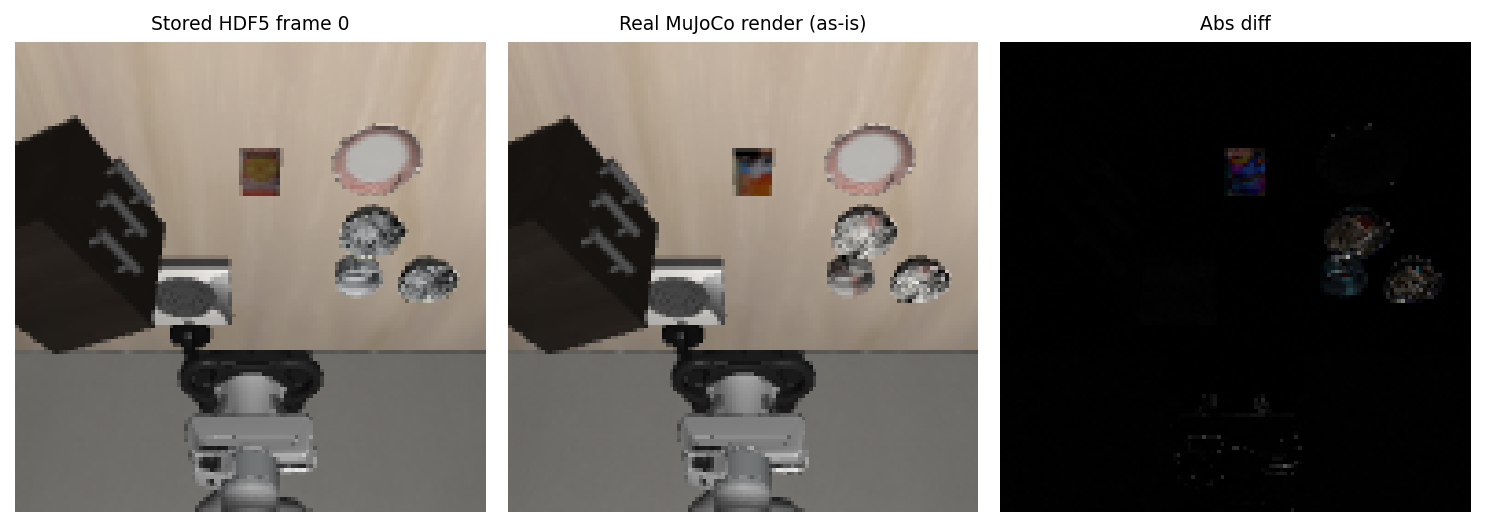
\includegraphics[width=0.85\textwidth]{figures/camera_verification.png}
  \caption{Frame 0 as stored in the HDF5 (left) vs.\ independently re-rendered from the live MuJoCo camera pose (center); the difference (right) is texture noise only.}
  \label{fig:camera_verification}
\end{figure}

\begin{figure}[htbp]
  \centering
  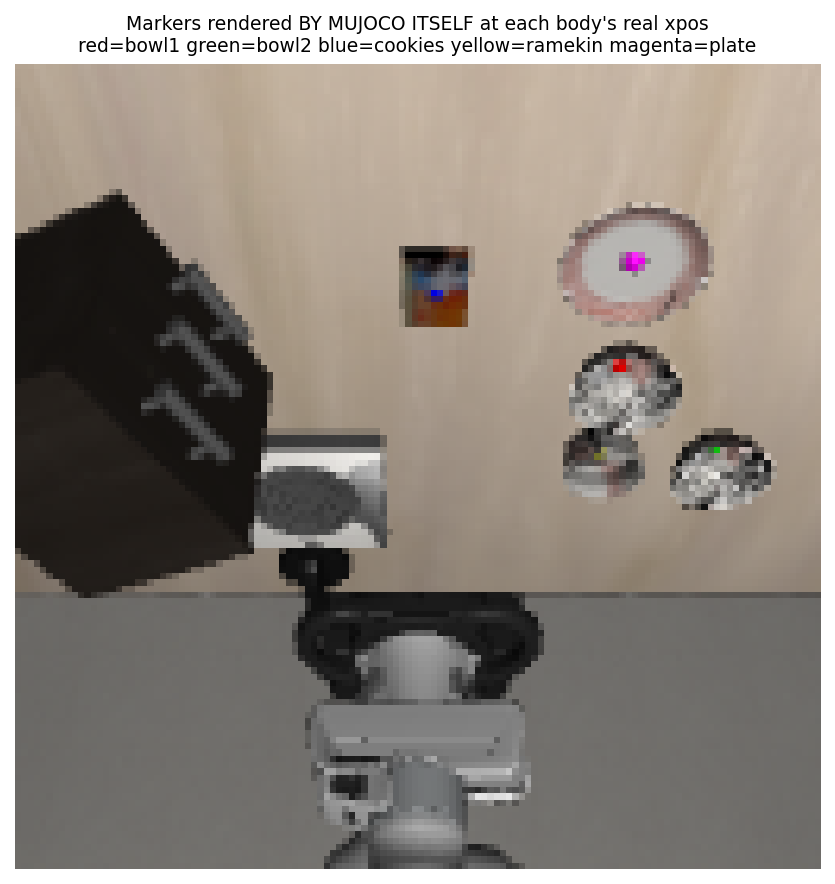
\includegraphics[width=0.55\textwidth]{figures/markers_in_scene.png}
  \caption{Markers rendered natively by MuJoCo at each object's true world position -- an independent ground-truth check on the projection pipeline.}
  \label{fig:markers_in_scene}
\end{figure}

\begin{figure}[htbp]
  \centering
  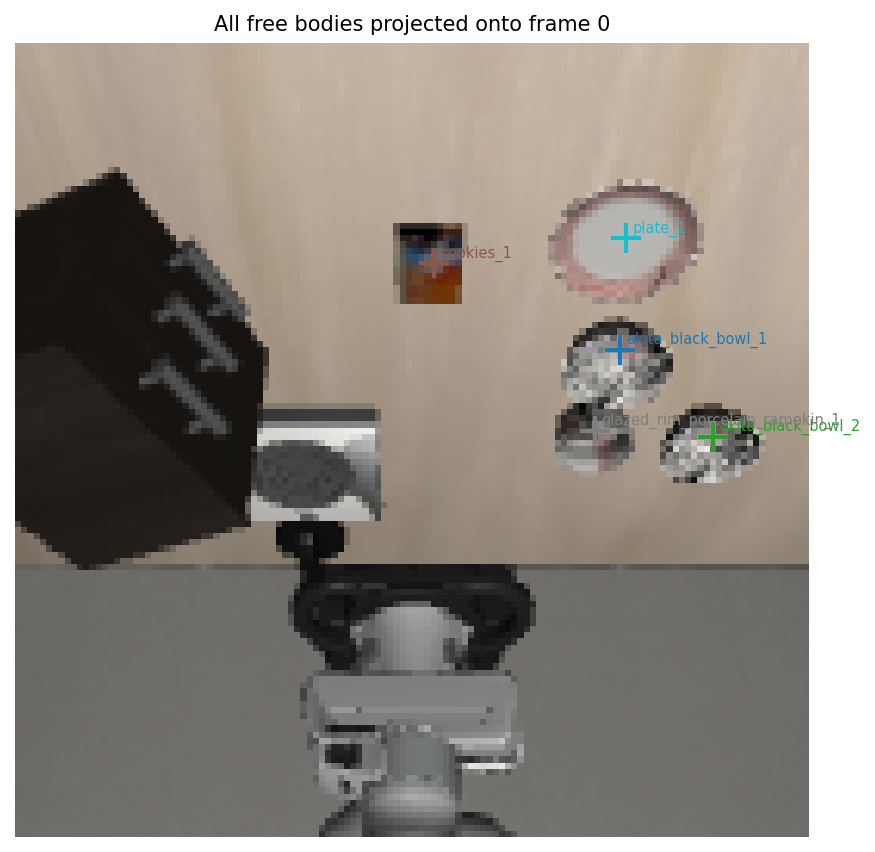
\includegraphics[width=0.55\textwidth]{figures/all_objects_projection.png}
  \caption{All five free bodies in the scene projected and labeled simultaneously, correctly distinguishing the two visually similar black bowls.}
  \label{fig:all_objects}
\end{figure}

\subsection{Annotation proof of concept}

The earliest end-to-end proof of concept confirmed, on the same frame, that the end-effector trajectory, a clean circle+arrow annotation, and a human-like wobbled variant all place the circle correctly on the target bowl among the plate/ramekin/cookie-box distractors, with the arrow correctly pointing from the bowl to the destination plate.

\subsection{Bugs found and fixed}

Building the full four-variant pipeline surfaced seven distinct issues, all resolved and re-verified:

\begin{enumerate}[nosep]
  \item \textbf{Time-travel bug}: an early version projected an object's grasp/release-frame position onto the frame-0 image. Fixed by standardizing all annotation ground truth on frame 0, matching what the human actually sees in the evaluation protocol (Section 3.1 of the proposal).
  \item \textbf{Visual-center offset}: for several object meshes (notably the bowls), the MuJoCo body origin sits at the object's base, not its visual center, biasing circle placement by roughly half the object's height. Fixed by preferring each body's non-colliding reference geom (or a measured local offset) over raw \texttt{body\_xpos}.
  \item \textbf{Row-mirroring convention}: the raw output of \texttt{robosuite}'s world-to-camera projection was vertically mirrored relative to the stored frame for this camera/robosuite/MuJoCo combination. Found and fixed by cross-checking against the MuJoCo-native marker ground truth (Figure~\ref{fig:markers_in_scene}).
  \item \textbf{Color-channel swap}: a refactor moved the RGB$\to$BGR color conversion to before, rather than after, the drawing step, silently turning every red arrow blue. Caught by directly sampling drawn pixel values rather than trusting a visual glance at a 128$\times$128 thumbnail.
  \item \textbf{Uninformative motion arrows}: the raw grasp$\to$release end-effector window sometimes ends well short of the object's true final resting position (the gripper releases before the object settles under gravity), producing arrows that visibly undershot the destination. Fixed by anchoring the final motion-arrow waypoint to the true destination centroid, so only the arrow's shape -- not its endpoint -- differs from the destination arrow.
  \item \textbf{Missing symbolic tokens}: an intermediate version of the pipeline dropped the symbolic-token representation entirely, silently regressing on proposal Section 2.5's two-representations requirement. Restored and extended (separate $r_x$/$r_y$ for the wobbled ellipse; a waypoint list for motion arrows).
  \item \textbf{Silent write truncation}: roughly 80\% of \texttt{motion\_arrow} PNGs were being written as truncated, undecodable files (missing the PNG \texttt{IEND} footer), while reporting success. Root cause: verifying a write by reading it back \emph{in the same process, immediately after writing} does not prove the bytes are durably flushed across the WSL2$\leftrightarrow$Windows filesystem bridge -- a same-process read can be satisfied by the OS page cache before the underlying file is actually complete on disk. Fixed by encoding the PNG fully in memory first, writing with an explicit \texttt{flush()} + \texttt{os.fsync()}, and verifying via a freshly-opened file handle checking exact byte length, the PNG end-of-file marker, and successful decode -- then independently re-verified from a second, physically separate mount of the same directory.
\end{enumerate}

\begin{figure}[htbp]
  \centering
  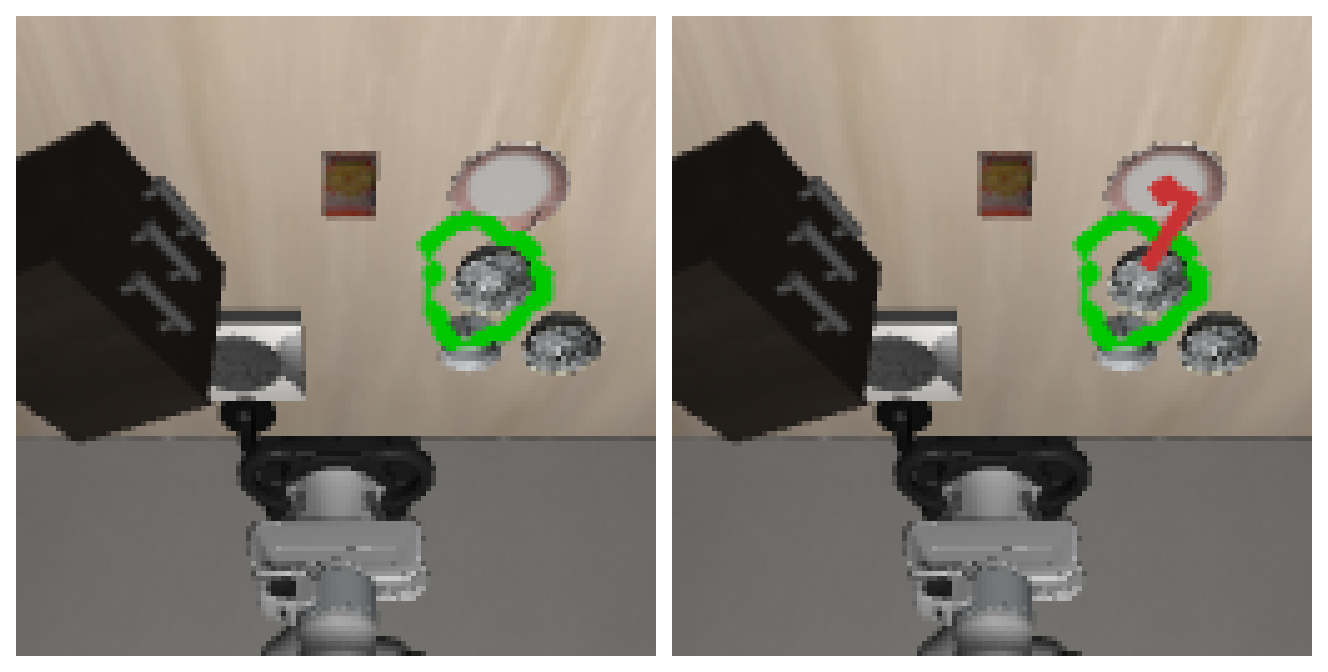
\includegraphics[width=0.75\textwidth]{figures/modality_variants_composite.png}
  \caption{Two of the four drawn variants for one demonstration, post-fix: circle only, and circle + destination arrow (correctly red). The circle + motion arrow variant is confirmed correct by the same checks (Section 3.4, item 7) but is omitted here as a figure since it could not be reliably re-transferred into this document at write time; its coordinates are recorded in \texttt{dataset\_metadata.json} under the \texttt{circle\_motion\_arrow} variant.}
  \label{fig:composite}
\end{figure}

\section{Contribution to the proposal}

This work directly delivers the feasibility argument at the core of Section 2: \emph{every training annotation can be generated automatically from simulator ground truth}, with no human labeling required. Concretely, it establishes three things the rest of the project depends on.

First, it validates that the camera and object-pose ground truth needed for pixel-accurate annotation is actually recoverable and correct, not just assumed -- which matters because the entire circle/arrow channel (proposal Section 1, the ``two minimal primitives'' thesis) is only as trustworthy as the pixels it is drawn from. Second, it produces the co-training data shape the proposal calls for in Section 2.4 -- clean text, ambiguous+circle, and ambiguous+circle+arrow -- as genuinely separate, correctly-labeled entries, which is the raw material Section 4.6's training recipe needs. Third, having both arrow flavors (destination and motion) generated as separate, parallel entries per demonstration rather than randomly choosing one keeps the door open for the destination-vs-motion ablation the proposal lists in Sections 4.3 and 4.5, without needing to regenerate the dataset later to get it.

\section{Limitations}

\begin{itemize}[nosep]
  \item \textbf{Scale}: the current dataset covers one task and five demonstrations. Nothing in the pipeline is task-specific, but it has not yet been run across the full LIBERO-Spatial suite, let alone Object/Goal/Long or LIBERO-90.
  \item \textbf{Caption degradation is templated, not general}: \texttt{degrade\_language\_referential} and \texttt{degrade\_language\_directional} currently return fixed strings (``pick up this one'', ``move this there'') regardless of the source instruction, rather than a general qualifier-stripping transformation. This is sufficient to manufacture ambiguity for a proof of concept but will not scale to more varied instructions without generalization.
  \item \textbf{No segmentation-mask reuse}: the proposal notes that LIBERO+/SlotVLA already publishes pixel-level masks that could be reused for circle fitting (Section 2.1). The current pipeline instead derives circle geometry from projected collision-geom bounding boxes, which is a reasonable proxy but not the same signal, and has not been cross-checked against LIBERO+ masks.
  \item \textbf{Motion-arrow endpoint is a deliberate simplification}: forcing the final waypoint to the true destination (Section 3, item 5) fixes the ``undershoot'' problem but slightly changes the arrow's semantics from ``the robot's literal path'' to ``the robot's approximate path, guaranteed to end at the goal.'' This is a reasonable and probably preferable choice for training signal quality, but it is a modeling decision worth flagging rather than a neutral bug fix.
  \item \textbf{No RLDS/HDF5 packaging yet}: annotations currently live as loose PNGs plus a JSON metadata file, not yet in the RLDS/HDF5 layout the proposal specifies for compatibility with the UniVLA data loader (Section 2.5, final paragraph).
  \item \textbf{Grasp/release detection has a known fallback}: the gripper-command heuristic occasionally fails to find a clean open$\to$close$\to$open transition, in which case a lower-confidence min-$z$ heuristic is used and motion-arrow generation is skipped for that demonstration. This has not yet been an issue in the five demonstrations processed, but its failure rate at full-dataset scale is unknown.
\end{itemize}

\section{Suggestions for Section 2.6 (negative and distractor mining)}

Section 2.6 asks for explicit hard cases: $N$ near-identical objects where only the circled instance is correct, and $M$ candidate destinations where only the arrow-pointed one is correct, over-represented relative to their natural frequency. Concretely, for this codebase:

\begin{itemize}[nosep]
  \item \textbf{The distractor case is already sitting in the data}: the verified scene in Figure~\ref{fig:all_objects} contains \emph{two} visually similar bowls, \texttt{akita\_black\_bowl\_1} and \texttt{akita\_black\_bowl\_2}, already correctly distinguished by the projection pipeline. The dataset generator currently only ever circles the BDDL-designated target; the natural next step is to also emit the non-target bowl's projected position as a labeled ``distractor'' object per demo, so downstream training/eval can construct (correct-circle, wrong-circle) pairs on the same frame.
  \item \textbf{LIBERO-Object is a more direct source of distractor-rich scenes} than LIBERO-Spatial, since its stated purpose is varying object identity against a fixed layout; it should be the primary suite for this subsection once distractor labeling logic exists.
  \item \textbf{Destination-side distractors} can reuse the same idea: LIBERO scenes with multiple plausible containers/regions (plate, drawer, stove, cabinet slots already visible in the downloaded LIBERO-Spatial files) give ready-made ``$M$ candidate destinations'' without needing new scenes -- the arrow should point at the BDDL-true one, with the others logged as hard negatives for a directional-accuracy metric.
  \item \textbf{Over-representation} is a sampling-time decision, not a generation-time one, given the current per-demo metadata schema: tag each entry with its distractor count and destination-candidate count at generation time, and control the training mixture via a weighted sampler, rather than duplicating hard cases physically in the dataset.
\end{itemize}

\end{document}
